\chapter{Directed graphs \& Partial Orders}\label{digraphs_chap}
%\section{Digraphs}\label{digraphs_sec}

\term{Directed graphs}, called \term{digraphs} for short, provide a
handy way to represent how things are connected together and how to
get from one thing to another by following those connections.  They are
usually pictured as a bunch of dots or circles with arrows between
some of the dots, as in Figure~\ref{fig:4N6E}.  The dots are called
\emph{nodes} or \emph{vertices} and the lines are called
\emph{directed edges} or \term{arrows}; the digraph in
Figure~\ref{fig:4N6E} has 4 nodes and 6 directed edges.

\begin{figure}

\graphic{Fig_EB}

\caption{A 4-node directed graph with 6 edges.}

\label{fig:4N6E}

\end{figure}

Digraphs appear everywhere in computer science.  For example, the
digraph in Figure~\ref{fig:6switchnet} represents a \idx{communication
  net}, a topic we'll explore in depth in Chapter~\ref{comm_net_chap}.
Figure~\ref{fig:6switchnet} has three ``in'' nodes (pictured as little
squares) representing locations where packets may arrive at the net,
the three ``out'' nodes representing destination locations for
packets, and the remaining six nodes (pictured with little circles)
represent switches.  The 16 edges indicate paths that packets can take
through the router.

\begin{figure}

\graphic{MQ_oct31_network}

\caption{A 6-switch packet routing digraph.}

\label{fig:6switchnet}
\end{figure}

Another place digraphs emerge in computer science is in the hyperlink
structure of the World Wide Web.  Letting the vertices $x_1, \dots,
x_n$ correspond to web pages, and using arrows to indicate when one
page has a hyperlink to another, results in a digraph like the one in
Figure~\ref{webpage-links}---although the graph of the real World Wide
Web would have $n$ be a number in the billions and probably even the
trillions.  At first glance, this graph wouldn't seem to be very
interesting.  But in 1995, two students at Stanford, \index{Page,
  Larry} Larry Page and \index{Brin, Sergey} Sergey Brin, ultimately
became multibillionaires from the realization of how useful the
structure of this graph could be in building a search engine.  So pay
attention to graph theory, and who knows what might happen!

\iffalse

and in the following graph the vertices $x_1, \ldots, x_n$ correspond
to web pages and $\diredge{x_i}{x_j}$ is a directed edge when page
$x_i$ contains a hyperlink to page $x_j$.
\fi


\begin{figure}

\graphic{randomWalkFigs/webGraph}

\caption{Links among Web Pages.}

\label{webpage-links}

\end{figure}
\begin{editingnotes}

The first line of this definition appeared on page 289; there was a
full page of diagrams before the rest of the definition appeared on
page 291. I added the samepage command here to fix it, hopefully it
won't have uninteded side-effects. -EM
\end{editingnotes}

\begin{samepage}
\begin{definition}\label{graphdef}
  A \term{directed graph}, $G$, consists of a nonempty
  set,~$\vertices{G}$, called the \term{vertices} of~$G$, and a set,
  $\edges{G}$, called the \term{edges} of $G$.  An element of
  $\vertices{G}$ is called a \term{vertex}.  A vertex is also called a
  \term{node}; the words ``vertex'' and ``node'' are used
  interchangeably.  An element of $\edges{G}$ is called a
  \term{directed edge}.  A directed edge is also called an ``arrow''
  or simply an ``edge.''  A directed edge \index{start
    vertex}{\emph{starts}} at some vertex, $u$, called the \term{tail}
  of the edge, and \index{end vertex}{\emph{ends}} at some vertex,
  $v$, called the \term{head} of the edge, as in Figure~\ref{fig:6EA}.
  Such an edge can be represented by the ordered pair $(u,v)$.  The
  notation $\diredge{u}{v}$ denotes this edge.
\end{definition}
\end{samepage}

\begin{figure}

\graphic{Fig_EA}

\caption{A directed edge $e = \diredge{u}{v}$.  The edge $e$ starts at
  the tail vertex, $u$, and ends at the head vertex, $v$.}

\label{fig:6EA}
\end{figure}

There is nothing new in Definition~\ref{graphdef} except for a lot of
vocabulary.  Formally, a digraph $G$ is the same as a binary relation
on the set, $V = \vertices{G}$---that is, a digraph is just a binary
relation whose domain and codomain are the same set, $V$.  In fact,
we've already referred to the arrows in a relation $G$ as the
``graph'' of $G$.  For example, the \idx{divisibility relation} on the
integers in the interval $[1,12]$ could be pictured by the digraph in
Figure~\ref{fig:divisibility-digraph}.

\section{Vertex Degrees}
The \term{in-degree} of a vertex in a digraph is the number of arrows
coming into it and similarly its \term{out-degree} is the number of
arrows out of it.  More precisely,
\begin{definition}\label{digraph-degree}
If $G$ is a digraph and $v \in \vertices{G}$, then
\begin{align*}
\indegr{v} \eqdef \card{\set{ e \in \edges{G} \suchthat \text{head}(e) = v}}\\
\outdegr{v} \eqdef \card{\set{ e \in \edges{G} \suchthat \text{tail}(e) = v}}\\
\end{align*}
\end{definition}

An immediate consequence of this definition is
\begin{lemma}\label{digraph-handshake}
\[
\sum_{v \in \vertices{G}} \indegr{v} = \sum_{v \in \vertices{G}} \outdegr{v}.
\]
\end{lemma}
\begin{proof}
Both sums are obviously equal to $\card{\edges{G}}$.
\end{proof}

\begin{problems}
\examproblems
\pinput{FP_outdegree_induction}
\end{problems}

\section{Walks and Paths}
Picturing digraphs with points and arrows makes it natural to talk
about following successive edges through the graph.  For example, in
the digraph of Figure~\ref{fig:divisibility-digraph}, you might start
at vertex 1, successively follow the edges from vertex 1 to vertex 2,
from 2 to 4, from 4 to 12, and then from 12 to 12 twice (or as many
times as you like).  The sequence of edges followed in this way is
called a \emph{walk} through the graph.

\begin{figure}
\graphic{divisibility}
\caption{The Digraph for Divisibility on $\set{1,2,\dots,12}$.}
\label{fig:divisibility-digraph}
\end{figure}

The obvious way to represent a walk is with the sequence of sucessive
vertices it went through, in this case:
\[
1\ \:2\ \:4\ \:12\ \:12\ \:12.
\]
However, it is conventional to represent a walk by an alternating
sequence of successive vertices and edges, so this walk would formally
be
\begin{equation}\label{walk12412}
1\ \diredge{1}{2}\  2\  \diredge{2}{4}\  4\ \diredge{4}{12}\  12\ 
\diredge{12}{12}\  12\ \diredge{12}{12}\  12.
\end{equation}\
The redundancy of this definition is enough to make any computer
scientist cringe, but it does make it easy to talk about how many
times vertices and edges occur on the walk.  Here is a formal
definition:

\begin{definition}\label{def:digraph-walks}
A \term{walk in a digraph}, $G$, is an alternating sequence of
vertices and edges that begins with a vertex, ends with a vertex, and
such that for every edge $\diredge{u}{v}$ in the walk, vertex $u$ is
the element just before the edge, and vertex $v$ is the next element
after the edge.

So a walk, $\walkv{v}$, is a sequence of the form
\[
\walkv{v} \eqdef v_0\ \diredge{v_0}{v_1}\
v_1\  \diredge{v_1}{v_2}\  v_2\  \dots\  \diredge{v_{k-1}}{v_k}\  v_k
\]
where $\diredge{v_i}{v_{i+1}} \in \edges{G}$ for $i \in [0,k)$.
  The walk is said to \emph{start} at $v_0$, to \emph{end} at $v_k$,
  and the \emph{length}, $\lnth{\walkv{v}}$, of the walk is defined to be
  $k$. 

 The walk is a \emph{path} iff all the $v_i$'s are different, that is,
 if $i \neq j$, then $v_i \neq v_j$.

A \term{closed walk} is a walk that begins and ends at the same
vertex.  A \term{cycle} is a closed walk whose vertices are distinct
except for the beginning and end vertices.
\end{definition}
Note that a single vertex counts as a length zero path, as well as a
length zero cycle, that begins and ends at itself.  Length-1 cycles
are possible when a node has an arrow leading back to itself.  The
graph in Figure~\ref{fig:4N6E} has none, but every vertex in the
divisibility relation digraph of Figure~\ref{fig:divisibility-digraph}
is in a length-1 cycle.  Length-1 cycles are sometimes called
\term{self-loops}.

Although a walk is officially an alternating sequence of vertices and
edges, it is completely determined just by the sequence of successive
vertices on it, or by the sequence of edges on it.  We will
describe walks in these ways whenever it's convenient.  For example,
for the graph in Figure~\ref{fig:4N6E},
\begin{itemize}

\item $(a, b, d)$, or simply $abd$, is a (vertex-sequence description
  of a) length-2 path,

\item $(\diredge{a}{b}, \diredge{b}{d})$, or simply
  $\diredge{a}{b}\diredge{b}{d}$, is (an edge-sequence description of)
  the same length-2 path,

\item $abcbd$ is a length-4 walk,

\item $dcbcbd$ is a length-5 closed walk,

\item $bdcb$ is a length-3 cycle,

\item $\diredge{b}{c}\diredge{c}{b}$ is a length-2 cycle, and

\item $\diredge{c}{b}\ang{b\! \leftarrow\! a}\diredge{a}{d}$
  is \emph{not} a walk.  A walk is not allowed to follow
  edges in the wrong direction.
\end{itemize}


\begin{editingnotes}
length~2 cycles are not possible with undirected graphs.
\end{editingnotes}

If you walk for a while, stop for a rest at some vertex, and then
continue walking, you have broken a walk into two parts.  For example,
stopping to rest after following two edges in the walk~\eqref{walk12412}
through the divisibility graph breaks the walk into the first part of the walk
\begin{equation}\label{startwalk124}
1\ \diredge{1}{2}\  2\  \diredge{2}{4}\  4
\end{equation}
from 1 to 4, and the rest of the walk
\begin{equation}\label{endwalk412}
4\ \diredge{4}{12}\  12\  \diredge{12}{12}\  12\ \diredge{12}{12}\  12.
\end{equation}
from 4 to 12, and we'll say the whole walk~\eqref{walk12412} is the
\term{merge} of the walks~\eqref{startwalk124} and~\eqref{endwalk412}.
In general, if a walk $\walkv{f}$ ends with a vertex, $v$, and a walk
$\walkv{r}$ starts with the same vertex, $v$, we'll say that their
\term{merge}, $\merge{\walkv{f}}{\walkv{r}}$, is the walk that starts
with $\walkv{f}$ and continues with $\walkv{r}$.\footnote{It's
  tempting to say the \emph{merge} is the \idx{concatenation} of the
  two walks, but that wouldn't quite be right because if the walks
  were concatenated, the vertex $v$ would appear twice in a row where
  the walks meet.}  Two walks can only be merged if the first ends
with the same vertex, $v$, that the second one starts with.  Sometimes
it's useful to name the node $v$ where the walks merge; we'll use the
notation $\catv{\walkv{f}}{v}{\walkv{r}}$ to describe the merge of a
walk $\walkv{f}$ that ends at $v$ with a walk $\walkv{r}$ that begins
at $v$.

\iffalse
 Here's a precise definition:
\begin{definition}
If a walk $\walkv{f}$ ends at a vertex $v$ and a walk $\walkv{r}$
begins at the same vertex $v$, then the \term{$v$-merge} of
$\walkv{f}$ with $\walkv{r}$, written,
\[
\catv{\walkv{f}}{v}{\walkv{r}},
\]
is the walk whose vertex sequence is the vertex sequence of
$\walkv{f}$ concatenated with the vertex sequence of $\walkv{r}$
without its initial $v$.  That is, if
\begin{align*}
\walkv{r} & = v\,\vec{\alpha},
\end{align*}
for some finite sequence $\vec{\alpha}$ of vertices,
then
\[
\catv{\walkv{f}}{v}{\walkv{r}} \eqdef  \walkv{f}\alpha.
\]
\end{definition}
\fi

A consequence of this definition is that
\begin{lemma}\label{sumoflengths}
\[
\lnth{\merge{\walkv{f}}{\walkv{r}}} = \lnth{\walkv{f}} + \lnth{\walkv{r}}.
\]
\end{lemma}
In the next section we'll get mileage out of walking this way.

\subsection{Finding a Path}
If you were trying to walk somewhere quickly, you'd know you were in
trouble if you came to the same place twice.  This is actually a basic
theorem of graph theory.

\begin{theorem}\label{shortestwalk_thm}
The shortest walk from one vertex to another is a path.
\end{theorem}

\begin{proof}
  If there is a walk from vertex $u$ to another vertex $v \neq u$,
  then by the Well Ordering Principle, there must be a minimum length
  walk $\walkv{w}$ from $u$ to~$v$.  We claim $\walkv{w}$ is a path.

  To prove the claim, suppose to the contrary that $\walkv{w}$ is not a
  path, meaning that some vertex $x$ occurs twice on this walk.  That is,
\[
\walkv{w} = \catv{\catv{\walkv{e}}{x}{\walkv{f}}}{x}{\walkv{g}}
\]
for some walks $\walkv{e}, \walkv{f}, \walkv{g}$ where the length of
$\walkv{f}$ is positive.  But then ``deleting'' $\walkv{f}$ yields a
strictly shorter walk
\[
\catv{\walkv{e}}{x}{\walkv{g}}
\]
from $u$ to $v$, contradicting the minimality of $\walkv{w}$.
\end{proof}

\iffalse

Actually, we proved something stronger:
\begin{corollary}\label{pathlewalk_cor}
For any walk in a digraph, there is a path starting and ending at the
same vertices as the walk and containing only edges in the walk.  Such
a path is necessarily no longer than the walk.
\end{corollary}
\fi

\begin{editingnotes}
Distance properties below \arm{inserted by arm}
\end{editingnotes}

\begin{definition}
  The \index{distance!between vertices} \emph{distance}
  $\dstuv{u}{v}$, in a graph from vertex $u$ to vertex $v$ is the
  length of a shortest path from $u$ to $v$.
\end{definition}

As would be expected, this definition of distance satisfies:
\begin{lemma}\label{lem:tri-ineq} [The Triangle Inequality]
\[
\dstuv{u}{v} \leq \dstuv{u}{x} + \dstuv{x}{v}
\]
for all vertices $u,v,x$ with equality holding iff $x$ is on a shortest
path from $u$ to $v$.
\end{lemma}
Of course, you might expect this property to be true, but distance has a
technical definition and its properties can't be taken for granted.
For example, unlike ordinary distance in space, the distance from $u$
to $v$ is typically different from the distance from $v$ to $u$.
So, let's prove the Triangle Inequality

\begin{proof}
  To prove the inequality, suppose $\walkv{f}$ is a shortest path from
  $u$ to $x$ and $\walkv{r}$ is a shortest path from $x$ to $v$.  Then
  by Lemma~\ref{sumoflengths}, $\catv{\walkv{f}}{x}{\walkv{r}}$ is a
  walk of length $\dstuv{u}{x} + \dstuv{x}{v}$ from $u$ to $v$, so
  this sum is an upper bound on the length of the shortest path from
  $u$ to $v$ by Theorem~\ref{shortestwalk_thm}.
\end{proof}

Proof of the ``iff'' is in Problem~\ref{TP_digraph_triangle_inequality}
  
Finally, the relationship between walks and paths extends to closed walks and
cycles:
\begin{lemma}\label{shortestclosedwalk_lem}
The shortest positive length closed walk through a vertex is a
positive length cycle through that vertex. \footnote{The proof is
  essentially the same as for Theorem~\ref{shortestwalk_thm}.  See
  Problem~\ref{PS_shortest_directed_closed_walk}.}
\end{lemma}

\begin{editingnotes}

\textbf{This section needs to be motivated before being included.}

\section{Strong Connectivity}

\begin{definition}
A digraph is \term{strongly connected} when there is a path from each
vertex to every other vertex.
\end{definition}

For example, the graph in Figure~%\ref{fig:6EB}
is not strongly connected since there is no directed path from
node~$b$ to node~$a$.  But if node~$a$ is removed, the resulting graph
would be strongly connected.

A digraph is \term{weakly connected} \iffalse or, more simply,
\emph{connected})\fi if there is a ``path'' from from each vertex to
every other vertex when edges can be crossed forwards or backwards.
For example, the graph in Figure~%\ref{fig:6EB}
is weakly connected.

More precisely, a graph $G$ is weakly connected iff the graph $H$ with
\begin{align*}
\vertices{H} = \vertices{G}, \text{and}\\
\edges{H} = \edges{G} \union \set{\diredge{v}{u} \suchthat \diredge{u}{v} \in \edges{G}},
\end{align*}
is strongly connected.  In other words $H = G \union G^{-1}$.
\end{editingnotes}

\section{Adjacency Matrices}\label{sec:adjacency-matrix-digraph}
If a graph, $G$, has $n$ vertices, $v_0,v_1,\dots, v_{n-1}$, a useful
way to represent it is with an $n \times n$ matrix of zeroes and ones
called its \term{adjacency matrix}, $A_G$.  The $ij$th
entry of the adjacency matrix,  $(A_G)_{ij}$, is 1 if there is an edge
from vertex $v_i$ to vertex $v_j$ and 0 otherwise.  That is,
\[
(A_G)_{ij} \eqdef \begin{cases} 1 & \text{if } \diredge{v_i}{v_j} \in
  \edges{G},\\
0 & \text{otherwise}.
\end{cases}
\]
For example, let $H$ be the 4-node graph shown in
Figure~\ref{fig:4N6E}.  Its adjacency matrix, $A_H$, is the $4 \times
4$ matrix:
\[
A_H =\begin{array}{c|cccc|}
  &  a & b & c & d \\ \hline
a &  0 & 1 & 0 & 1 \\
b &  0 & 0 & 1 & 1 \\
c &  0 & 1 & 0 & 0 \\
d &  0 & 0 & 1 & 0
\end{array}
\]

A payoff of this representation is that we can use matrix powers to
count numbers of walks between vertices.  For example, there are two
length-2 walks between vertices $a$ and $c$ in the graph $H$:
\begin{align*}
a\ \diredge{a}{b}\ b\ \diredge{b}{c}\  c\\
a\ \diredge{a}{d}\ d\ \diredge{d}{c}\ c
\end{align*}
and these are the only length-2 walks from $a$ to $c$.  Also, there is
exactly one length-2 walk from $b$ to $c$ and exactly one length-2
walk from $c$ to $c$ and from $d$ to $b$, and these are the only
length-2 walks in $H$.  It turns out we could have read these counts
from the entries in the matrix $(A_H)^2$:
\[
(A_H)^2 = \begin{array}{c|cccc|}
  &  a & b & c & d \\ \hline
a &  0 & 0 & 2 & 1 \\
b &  0 & 1 & 1 & 0 \\
c &  0 & 0 & 1 & 1 \\
d &  0 & 1 & 0 & 0
\end{array}
\]

\iffalse
If $G$ is a weighted graph with edge weights given by $w: E \to
\reals$, then the adjacency matrix for~$G$ is $A_G = \{ a_{ij} \}$
where
\begin{equation*}
    a_{ij} = \begin{cases}
                w(\edge{v_i}{v_j}) & \text{if $\edge{v_i}{v_j} \in E$} \\
                0                 & \text{otherwise.}
              \end{cases}
\end{equation*}
\end{definition}

For example, Figure~\ref{fig:adjacency_matrix} displays the adjacency
matrices for the graphs shown in Figures~\ref{fig:isomorphism}(a)
and~\ref{fig:weighted_graph} where $v_1 = a$, $v_2 = b$, $v_3 = c$,
and $v_4 = d$.
\fi

More generally, the matrix $(A_G)^k$ provides a count of the number of
length $k$ walks between vertices in any digraph, $G$, as we'll now
explain.

\begin{definition}
  The length-$k$ \term{walk counting matrix} for an $n$-vertex graph $G$
  is the $n \times n$ matrix $C$ such that
\begin{equation}\label{def:walk_matrix}
C_{uv} \eqdef \text{the number of length-$k$ walks from $u$ to $v$}.
\end{equation}
\end{definition}
Notice that the adjacency matrix $A_G$ is the length-$1$ walk counting
matrix for $G$, and that$(A_G)^0$, which by convention is the identity
matrix, is the length-0 walk counting matrix.

\begin{theorem}\label{thm:CkDm}
 If $C$ is the length-$k$ walk counting matrix for a graph $G$, and
 $D$ is the length-$m$ walk counting matrix, then $CD$ is the length
 $k+m$ walk counting matrix for $G$.
\end{theorem}

According to this theorem, the square $(A_G)^2$ of the adjacency
matrix is the length-2 walk counting matrix for $G$.  Applying the
theorem again to $(A_G)^2A_G$, shows that the length-3 walk counting
matrix is $(A_G)^3$.  More generally, it follows by induction that
\begin{corollary}\label{AGklenk}
The length-$k$ counting matrix of a digraph, $G$, is $(A_G)^k$, for
all $k \in \naturals$.
\end{corollary}
In other words, you can determine the number of length~$k$ walks
between any pair of vertices simply by computing the $k$th power of
the adjacency matrix!   \iffalse

For example, the first three powers of the adjacency matrix for the
graph in Figure~\ref{fig:5AD} are:
\begin{align*}
    A &= \begin{pmatrix}
            0 & 1 & 1 & 1 \\
            1 & 0 & 1 & 0 \\
            1 & 1 & 0 & 1 \\
            1 & 0 & 1 & 0
         \end{pmatrix} & % \\[\medskipamount]
  A^2 &= \begin{pmatrix}
            3 & 1 & 2 & 1 \\
            1 & 2 & 1 & 2 \\
            2 & 1 & 3 & 1 \\
            1 & 2 & 1 & 2
         \end{pmatrix} & % \\[\medskipamount]
  A^3 &= \begin{pmatrix}
            4 & 5 & 5 & 5 \\
            5 & 2 & 5 & 2 \\
            5 & 5 & 4 & 5 \\
            5 & 2 & 5 & 2
         \end{pmatrix}
\end{align*}

Sure enough, $(A^3)_{14}$ is $5$, which is the number of length~3 walks
from~$v_1$ to~$v_4$.  And $(A^3)_{24} = 2$, which is the number of
length~3 walks from $v_2$ to~$v_4$.  
\fi

That may seem amazing, but the proof uncovers this simple relationship
between matrix multiplication and numbers of walks.

\begin{editingnotes}
\arm{new proof replacing induction proof by ftl}
\end{editingnotes}

\begin{proof}[Proof of Theorem~\ref{thm:CkDm}]
  Any length-$(k+m)$ walk between vertices $u$ and $v$ begins with a
  length-$k$ walk starting at $u$ and ending at some vertex, $w$,
  followed by a length-$m$ walk starting at $w$ and ending at $v$.  So
  the number of length-$(k+m)$ walks from $u$ to $v$ that go through
  $w$ at the $k$th step equals the number $C_{uw}$ of length-$k$ walks
  from $u$ to $w$, times the number $D_{wv}$ of length-$m$ walks from
  $w$ to $v$.  We can get the total number of length-$(k+m)$ walks
  from $u$ to $v$ by summing, over all possible vertices $w$, the
  number of such walks that go through $w$ at the $k$th step.  In
  other words,
\begin{equation}\label{ln+nuv}
\text{\#length-$(k+m)$ walks from $u$ to $v$} =
              \sum_{w \in \vertices{G}} C_{uw}\cdot D_{wv}
\end{equation}
But the right hand side of~\eqref{ln+nuv} is precisely the definition of
$(CD)_{uv}$.  Thus, $CD$ is indeed the length-$(k+m)$ walk counting matrix.
\end{proof}


\subsection{Shortest Paths}
The relation between powers of the adjacency matrix and numbers of
walks is cool---to us math nerds at least---but a much more important
problem is finding \index{graph!shortest path} shortest paths between
pairs of nodes.  For example, when you drive home for vacation, you
generally want to take the shortest-time route.

One simple way to find the lengths of all the shortest paths in an
$n$-vertex graph, $G$, is to compute the successive powers of $A_G$
one by one up to the $n-1$st, watching for the first power at which
each entry becomes positive.  That's because Theorem~\ref{thm:CkDm}
implies that the length of the shortest path, if any, between $u$
and~$v$, that is, the distance from $u$ to $v$, will be the smallest
value~$k$ for which $(A_G)_{uv}^k$ is nonzero, and if there is a
shortest path, its length will be $\leq n-1$.  Refinements of this
idea lead to methods that find shortest paths in reasonably efficient
ways.  The methods apply as well to weighted graphs, where edges are
labelled with weights or costs and the objective is to find least
weight, cheapest paths.  These refinements are typically covered in
introductory algorithm courses, and we won't go into them any
further.

\begin{editingnotes}
\textbf{Add this in the text or maybe some problems:}

\begin{definition}\label{def:5H}
  The \index{path!weight of}\term{weight of a walk} \index{weighted graph,
    path weight} in a \idx{weighted graph} is the sum of the weights of
  the successive edges in the walk.
\end{definition}

\arm{cut}
There is good news and bad news to report on this front.  The good
news is that it is not very hard to find a shortest path.  The bad
news is that you can't win one of those million dollar prizes for
doing it.

In fact, there are several good algorithms known for finding a shortest
path between nodes $u$ and $v$ in an $n$-node graph $G$.  The simplest to
explain (but not quite the fastest) is to compute \arm{revised to include
  stopping condition at $n$} the successive powers of $A_G$ one by one up
to the $n$th, watching for the first power at which the $uv$th entry is
nonzero.  That's because Theorem~\ref{thm:CkDm} implies that the length of
the shortest path, if any, between $u$ and~$v$ will be the smallest
value~$k$ for which $(A_G)_{uv}^k$ is nonzero, and if there is a shortest
path, its length will be $\leq n$.

\begin{definition}
  The \term{minimum weight matrix} for length $k$ walks in an $n$-vertex
  graph $G$ is the $n \times n$ matrix $W$ such that for $u,v \in \vertices{G}$,
\begin{equation}\label{def:weight_matrix}
W_{uv} \eqdef
\begin{cases} w & \text{if $w$ is the minimum weight among length $k$
                            walks from $u$ to $v$},\\
              \infty & \text{if there is no length $k$ walk from $u$ to $v$}.
\end{cases}
\end{equation}
\end{definition}

So the minimum weight matrix for length $1$ walks in a weighted graph $G$
is precisely its adjacency matrix $A_G$.  Now for the purpose of finding
minimum weight walks, we'll modify the definition of matrix
multiplication, replacing multiplication of elements by addition, and the
sum of the products by the minimum.

\arm{generalize to rectangular?}

\begin{definition}\label{def:minplus}
  The $\minplus$ product of two $n\times n$ matrices $W$ and $M$ with
  entries in $\reals\union \set{\infty}$ is the $n \times n$ matrix
  $W\minplusop M$ whose $ij$ entry is
\[
(W\minplusop M )_{ij} \eqdef \min \set{W_{ik} + M_{kj} \suchthat 1 \leq k \leq n}\, .
\]
\end{definition}

\begin{theorem}\label{thm:weightmatrix-min+}
  If $W$ is the minimum weight matrix for length $k$ walks in a weighted
  graph $G$, and $M$ is the minimum weight matrix for length $m$ walks,
  then then $W\minplusop M$ is the minimum weight matrix for length $k+m$
  walks.
\end{theorem}

\begin{proof}
  The proof is virtually the same as the proof of Theorem~\ref{thm:CkDm}
  with multiplication of elements replaced by addition, and the sum of the
  multiplications by the minimum of the additions:

  Any length $k+m$ path between vertices $u$ and $v$ begins with a length
  $k$ path starting at $u$ and ending at some vertex, $x$, followed by a
  length $m$ path starting at $x$ and ending at $v$.  So the minimum
  weight of a length $k+m$ path from $u$ to $v$ that goes through $x$ at
  the $k$th step equals the minimum weight $W_{ux}$ of length $k$ walks
  from $u$ to $x$, plus the minimum weight $M_{xv}$ of length $m$ walks
  from $w$ to $v$.  So we can get the minimum weight of length $k+m$ walks
  from $u$ to $v$ by taking the minimum over all possible vertices $x$ of
  the minimum weight of such walks that go through $w$ at the $k$th step.
  In other words,
\begin{equation}\label{ln-min+nuv}
\text{min weight of a length $n+m$ path from $u$ to $v$} =
              \min_{x \in \vertices{G}} W_{ux}+M_{xv}\, .
\end{equation}
But the right hand side of~\eqref{ln-min+nuv} is precisely the definition of
$(W\minplusop M)_{uv}$.  Thus, $W\minplusop M$ is indeed the minimum weight
matrix for walks of length $k+m$.
\end{proof}

Now Theorem~\ref{thm:weightmatrix-min+} implies that the $k$th $\minplus$ power
of $A_G$, that is,
\[
(A_G)^{k, \minplus} \eqdef \underbrace{\paren{A_G\ \minplusop\ \paren{A_G\
      \minplusop\ \paren{\cdots \paren{A_G\ \minplusop\ A_G}} }}}_{k\ A_G\text{'s}},
\]
is the minimum weight matrix for the length $k$ walks.

This takes us most of the way, but we really want the minimum weight
regardless of the lengths of the walks.  To get this, we use the fact that
as long as all weights are \emph{nonnegative}, the minimum weight walk
between two vertices will be a path; this follows by the same reasoning
used for Theorem~\ref{shortestwalk_thm}.  Since $n-1$ is the longest \emph{path}
can be in an $n$-node graph, we have an upper bound on the length of
minimum weight paths we have to look at.  We could now find the minimum
weight paths by computing all the $\minplus$ powers of $A_G$ up to the
$n-1$st.  But there is another trick that dramatically cuts the number of
$\minplus$ matrix multiplications.

Namely, for any graph $G$, let $G_0$ be the same as $G$ except that
self-loops of weight zero appear at every vertex.  So a path of length $k$
in $G$ can be extended to a path in $G_0$ with the same weight but with
any desired length $ \geq k$---just repeatedly follow weight zero
self-loops after the $k$th step.  This means that $(A_{G_0})^{k, \minplus}$
is the minimum weight matrix for walks of length \emph{less than or equal}
to $k$ in $G$.  So we can choose $k = n-1$ to get a matrix with the
actual minimum weights among all walks between vertices.

\begin{theorem}\label{thm:minweightmatrix}
Let $G$ be an $n$-vertex weighted graph with nonnegative weights, and let
$D_G$ be the adjacency matrix of $G$ with the diagonal entries set to 0.
Then $(D_G)^{n-1, \minplus}$ is the minimum weight path matrix for $G$, that
is,
\[
((D_G)^{n-1, \minplus})_{uv} = \text{the minimum weight of walks in $G$ from
 $u$ to $v$}\,.
\]
\end{theorem}
Now you can use the repeated squaring trick to compute $(D_G)^{n-1,
  \minplus}$ with only $\log n$ $\minplus$ matrix multiplications
instead of $n-2$ such multiplications.

\arm{Good to add an example here}
\end{editingnotes}

\section{Walk Relations}\label{walk_relation_sec}
A basic question about a digraph is whether there is a way to get from one
particular vertex to another.  So for any digraph, $G$, we are
interested in a binary relation, $G^*$, called the \term{walk
  relation} on $\vertices{G}$ where
\begin{equation}\label{G*def}
u \mrel{G^*} v \eqdef \mbox{there is a walk in $G$ from $u$ to $v$}.
\end{equation}
Similarly, there is a \term{positive walk relation}
\begin{equation}\label{G+def}
u \mrel{G^+} v \eqdef \mbox{there is a positive length walk in $G$ from 
$u$ to $v$}.
\end{equation}

\begin{definition}
When there is a walk from vertex $v$ to vertex $w$, we say that $w$ is
\term{reachable} from $v$, or equivalently, that $v$ is
\term{connected} to $w$.
\end{definition}

\subsection{Composition of Relations}\label{relation_compose_subsec}
There is a simple way to extend \idx{composition} of functions to
composition of relations, and this gives another way to talk about
walks and paths in digraphs.

\begin{definition}
Let $R: B\to C$ and $S: A \to B$ be binary relations.  Then the
\idx{composition} of $R$ with $S$ is the binary relation $(R \compose
S): A\to C$ defined by the rule
\begin{equation}\label{rel_compose_def}
a \mrel{(R \compose S)} c \eqdef\ \exists b \in B.\, (a \mrel{S} b)
\QAND (b \mrel{R} c).
\end{equation}
This agrees with the Definition~\ref{func_compose_def} of composition
in the special case when $R$ and $S$ are functions.\footnote{The
  reversal of the order of $R$ and $S$ in~\eqref{rel_compose_def} is
  not a typo.  This is so that relational composition generalizes
  function composition.  The value of function $f$ composed with
  function $g$ at an argument, $x$, is $f(g(x))$.  So in the
  composition, $f \compose g$, the function $g$ is applied first.}
\end{definition}

\begin{editingnotes}

\footnote{Some texts define $R \compose S$ the other way around, that
  is, with $S$ applied to the result of applying $R$ first.}

\end{editingnotes}

Remembering that a digraph is a binary relation on its vertices, it
makes sense to compose a digraph $G$ with itself.  Then if we let
$G^n$ denote the composition of $G$ with itself $n$ times, it's easy
to check (see Problem~\ref{CP_walk_relation_composition}) that $G^n$
is the \term{length-$n$ walk relation}:
\[
a  \mrel{G^n} b \qiff \mbox{ there is a length-$n$ walk in $G$ from $a$ to $b$}.
\]
This even works for $n=0$, with the usual convention that $G^0$ is the
identity relation $\ident{\vertices{G}}$ on the set of
vertices.\footnote{The identity relation, $\ident{A}$, on a set, $A$,
  is the equality relation:
\[
a \mrel{\ident{A}} b \qiff a  = b,
\]
for $a,b \in A$.}  Since there is a walk iff there is a path,
and every path is of length at most $\card{\vertices{G}}-1$, 
we now have\footnote{Equation~\eqref{g*union} involves a harmless
  abuse of notation: we should have written
\[
\graph{G^*} = \graph{G^0} \union \graph{G^1} \dots.
\]
}
\begin{equation}\label{g*union}
G^* = G^0 \union G^1 \union G^2 \union \dots \union
G^{\card{\vertices{G}}-1} = (G \union G^0)^{\card{\vertices{G}}-1}.
\end{equation}
The final equality points to the use of repeated squaring as a way to
compute $G^*$ with $\log n$ rather than $n-1$ compositions of
relations.

\begin{problems}
\practiceproblems
\pinput{TP_Composition_of_Relations}
\pinput{TP_digraph_triangle_inequality}

\homeworkproblems
\pinput{PS_relation_matrices}
\end{problems}

\section{Directed Acyclic Graphs \& Scheduling}\label{dag_sec}

Some of the prerequisites of MIT computer science subjects are shown
in Figure~\ref{6-3_subjects}.  An edge going from subject $s$ to
subject $t$ indicates that $s$ is listed in the catalogue as a direct
prerequisite of $t$.  Of course, before you can take subject $t$, you
have to take not only subject $s$, but also all the prerequisites of $s$,
and any prerequisites of those prerequisites, and so
anon.
\begin{editingnotes} Of course, in order to take subject $t$, you
  not only have to take subject $s$ first, but you also have to take
  all the prerequisites of $s$, as well as any prerequisites of these
  prerequisites, and so on.
\end{editingnotes}
We can state this precisely in terms of the positive walk relation: if
$D$ is the direct prerequisite relation on subjects, then subject $u$
has to be completed before taking subject $v$ iff $u \mrel{D^+} v$.

\begin{figure}

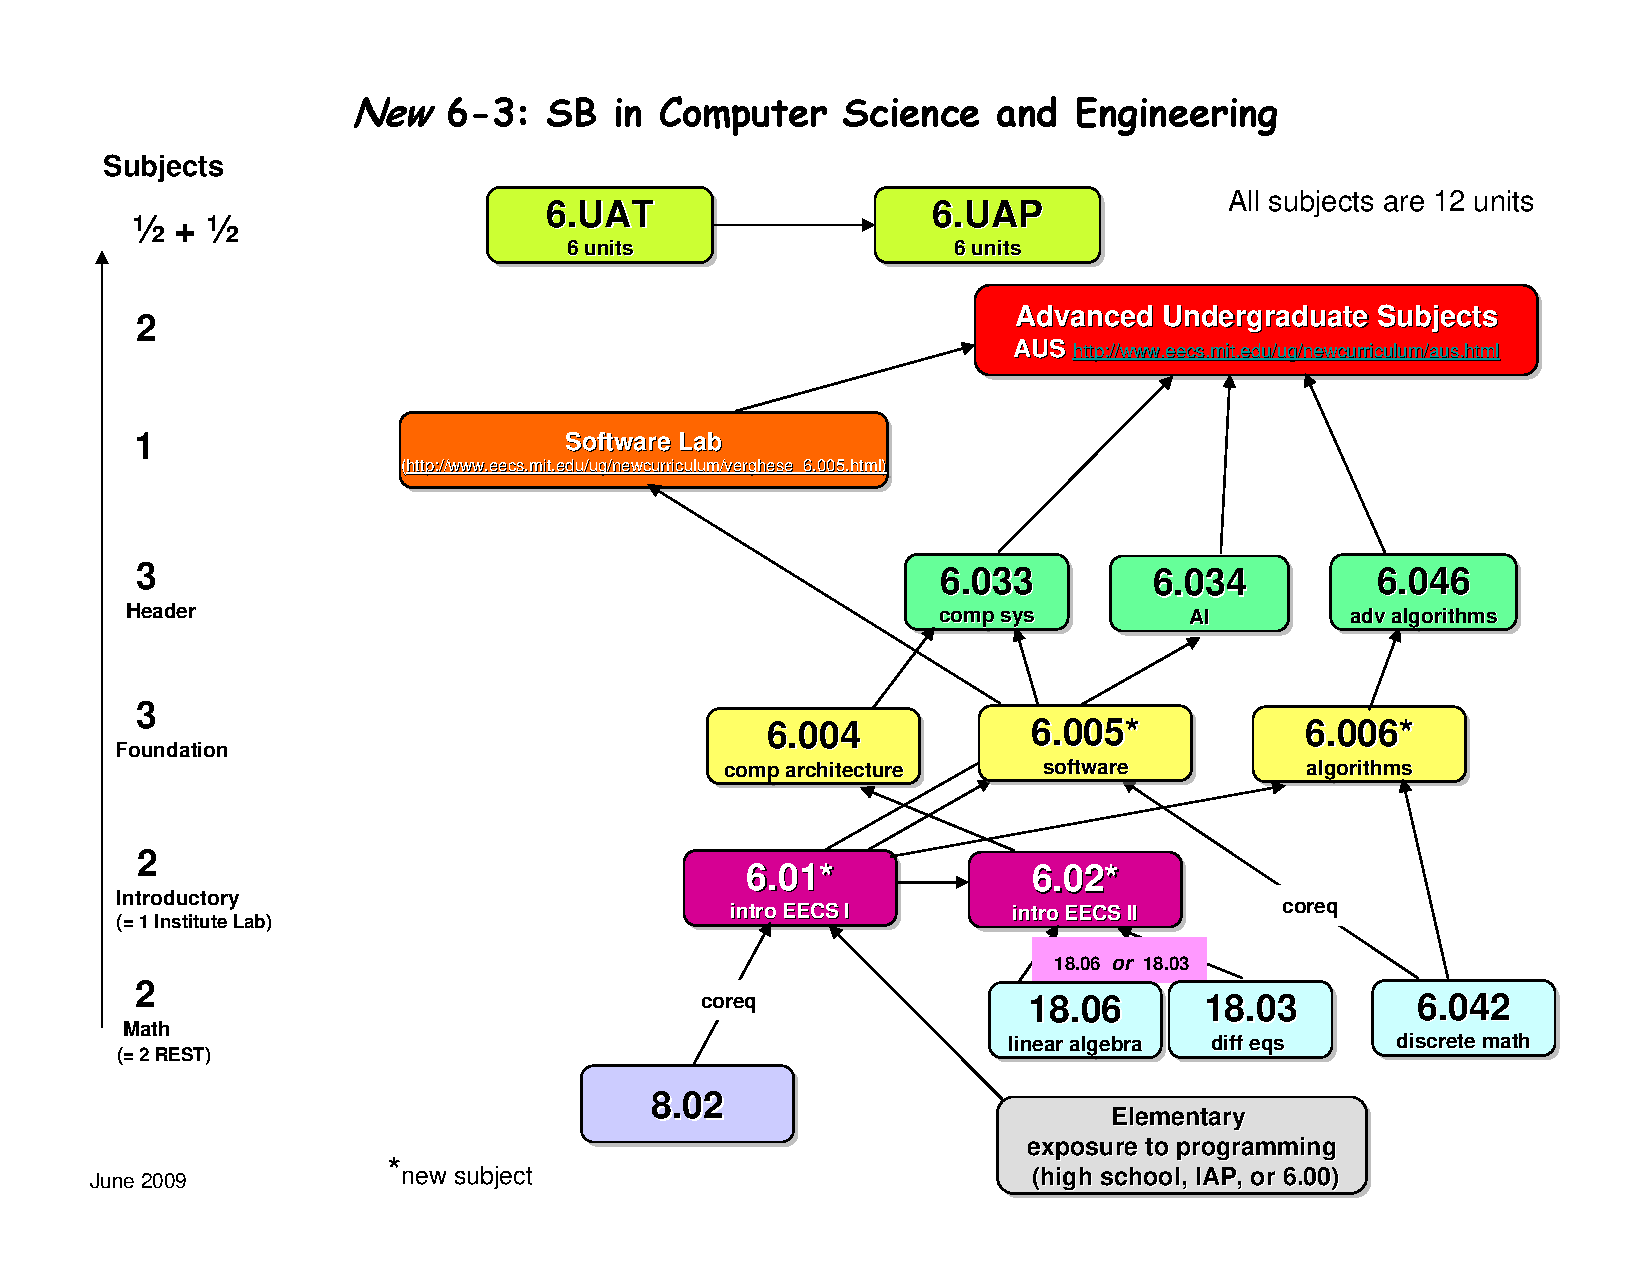
\includegraphics[width = 5in]{6-3_dag}

\caption{Subject prerequisites for MIT Computer Science (6-3) Majors.}

\label{6-3_subjects}

\end{figure}

It would clearly have a dire effect on the time it takes to graduate
if this direct prerequisite graph had a positive length closed walk.
We need to forbid such closed walks, which, by
Lemma~\ref{shortestclosedwalk_lem} is the same as forbidding positive
length cycles.  So, the direct prerequisite graph among subjects had
better be \term{acyclic}:

\begin{definition}
A \term{directed acyclic graph (DAG)} is a directed graph with no
positive length cycles.
\end{definition}

DAGs have particular importance in computer science.  They capture key
concepts used in analyzing task scheduling and concurrency control.
When distributing a program across multiple processors, we're in
trouble if one part of the program needs an output that another part
hasn't generated yet!  So let's examine DAGs and their connection to
scheduling in more depth.

\iffalse
We won't be working on any examples quite so
technical in this chapter, but\fi


%% Scheduling %%%%%%%%%%%%%%%%%%%%%%%%%%%%%%%%%%%%%%%%%%%%%%%%%%%%%%%%%%%%%%%%%
\subsection{Scheduling}\label{sched_subsec}

In a scheduling problem, there is a set of tasks and a set of
constraints specifying that starting a certain task depends on other
tasks being completed beforehand.  We can map this task to a digraph,
with the tasks as the nodes and the direct prerequisite constraints as
the edges.

For example, the DAG in Figure~\ref{fig:7FP} describes how a man might
get dressed for a formal occasion.  As we describe above, vertices
correspond to garments and the edges specify which garments have to be
put on before which others.

\begin{figure}

\graphic{Fig_FP}

\caption{DAG describing which clothing items have to be put on before others.}

\label{fig:7FP}

\end{figure}

When faced with a set of prerequisites like this one, the most basic
task is finding an order in which to perform all the tasks, one at a
time, while respecting the dependency constraints.  Ordering tasks in
this way is known as \emph{topological sorting}.

\begin{definition}
  A \term{topological sort} of a finite DAG is a list of all the
  vertices such that each vertex $v$ appears earlier in the list than
  every other vertex reachable from $v$.
\end{definition}

\begin{figure}\redrawntrue

\begin{tabular}{c@{\hspace{4em}}c}
underwear       & left sock \\
shirt           & shirt \\
pants           & tie \\
belt            & underwear \\
tie             & right sock \\
jacket          & pants \\
left sock       & right shoe \\
right sock      & belt \\
left shoe       & jacket \\
right shoe      & left shoe \\[\medskipamount]
(a)             & (b)
\end{tabular}

\caption{Two possible topological sorts of the prerequisites described in
  Figure~\ref{fig:7FP}}.
\label{fig:7FQ}
\end{figure}

There are many ways to get dressed one item at a time while obeying
the constraints of Figure~\ref{fig:7FP}.  We have listed two such
topological sorts in Figure~\ref{fig:7FQ}.  In fact, we can
prove that \emph{every} finite DAG has a topological sort.  You can
think of this as a mathematical proof that you can indeed get dressed
in the morning.
%(and then show up for math lecture).

Topological sorts for finite DAGs are easy to construct by starting
from \term{minimal} elements:

\begin{definition}
  An vertex $v$ of a DAG, $D$, is
  \index{minimum}\term*{minim\underline{um}} iff every other vertex is
  reachable from $v$.

  A vertex $v$ is \index{minimal}\term*{minim\underline{al}} iff $v$
  is not reachable from any other vertex.
\end{definition}

It can seem peculiar to use the words ``minimum'' and ``minimal'' to
talk about vertices that start paths.  These words come from the
perspective that a vertex is ``smaller'' than any other vertex it
connects to.  We'll explore this way of thinking about DAGs in the
next section, but for now we'll use these terms because they
are conventional.

\iffalse
In a topological sort, minimum and minimal elements are the same thing.
\fi

A DAG may have no minimum element but lots of minimal elements.  There
are four minimal elements in the clothes example: leftsock, rightsock,
underwear, and shirt.

To build an order for getting dressed, we pick one of these minimal
elements---say, shirt.  Now there is a new set of minimal elements;
the three elements we didn't chose as step 1 are still minimal, and once
we have removed shirt, tie becomes minimal as well.  We pick
another minimal element, continuing in this way until all elements
have been picked.  The sequence of elements in the order they were
picked will be a topological sort.  This is how the topological sorts
above were constructed.

\begin{editingnotes}
\textcolor{red}{pedantic lemma}

For this method of topological sorting to work, we need to be sure
there is always a minimal element.  This is sort of obvious, but
noting that an infinite partially ordered set might have no minimal
element---consider $<$ on the $\integers$---we'll practice doing an
elementary proof about partial orders by proving that minimal elements
exist.

\begin{lemma}\label{finmin}
  \hyperdef{rule}{mine1}{Every} partial order on a nonempty finite set
  has a minimal element.

\begin{proof} Let $R$ be a strict partial order on a set, $A$.  Define
 the \emph{weight}of an element $a \in A$ to be
 $\card{R\set{a}}$---the number of elements in the set $R\set{a}$.
 Since $A$ is finite, the weights of all elements in $A$ are
 nonnegative integers, so by well ordering, there must be an $a_0 \in
 A$ with the smallest weight.

Now suppose $\card{R\set{a_0}} \neq 0$.  Then there is an element $a_1 \in
R\set{a_0}$, which implies (by transitivity of $R$) that $R\set{a_1}
\subseteq R\set{a_0}$, and hence $\card{R\set{a_1}} \leq
\card{R\set{a_0}}$.  But since $R$ is strict, $a_1 \in R\set{a_0} -
R\set{a_1}$, so in fact $\card{R\set{a_1}} < \card{R\set{a_0}}$,
contradicting the fact the $a_0$ has the smallest weight.

This contradiction implies that $\card{R\set{a_0}} = 0$, which means that
no element is related by $R$ to $a_0$, that is, $a_0$ is minimal.

A similar argument works in the case that $R$ is a weak partial order.

\end{proof}
\end{lemma}

\end{editingnotes}

So our construction shows:

\begin{theorem}\label{thm:topological}
Every finite DAG has a topological sort.
\end{theorem}

There are many other ways of constructing topological sorts.  For
example, instead of starting from the minimal elements at the
beginning of paths, we could build a topological sort starting from
\term{maximal} elements at the end of paths.  In fact, we could build
a topological sort by picking vertices arbitrarily from a finite DAG
and simply inserting them into the list wherever they will
fit.\footnote{In fact, the DAG doesn't even need to be finite, but
  you'll be relieved to know that we have no need to go into this.}

\subsection{Parallel Task Scheduling}\label{parallel_sec}

For task dependencies, topological sorting provides a
way to execute tasks one after another while respecting those dependencies.
But what if we have the ability to execute more than one task at the same
time?  For example, say tasks are programs, the DAG indicates
data dependence, and we have a parallel machine with lots of processors
instead of a sequential machine with only one.  How should we schedule the
tasks?  Our goal should be to minimize the total \emph{time} to complete
all the tasks.  For simplicity, let's say all the tasks take the same
amount of time and all the processors are identical.

So given a finite set of tasks, how long does it take to do them all
in an optimal parallel schedule?  We can use walk relations on
acyclic graphs to analyze this problem.

In the first unit of time, we should do all minimal items, so we would
put on our left sock, our right sock, our underwear, and our
shirt.\footnote{Yes, we know that you can't actually put on both socks
  at once, but imagine you are being dressed by a bunch of robot
  processors and you are in a big hurry.  Still not working for you?
  Ok, forget about the clothes and imagine they are programs with the
  precedence constraints shown in Figure~\ref{fig:7FP}.}  In the
second unit of time, we should put on our pants and our tie.  Note
that we cannot put on our left or right shoe yet, since we have not
yet put on our pants.  In the third unit of time, we should put on our
left shoe, our right shoe, and our belt.  Finally, in the last unit of
time, we can put on our jacket.  This schedule is illustrated in
Figure~\ref{fig:7FS}.

\begin{figure}

\graphic{Fig_FS}

\caption{A parallel schedule for the tasks-getting-dressed digraph in
Figure~\ref{fig:7FP}.  The tasks in~$A_i$ can be performed in step~$i$
for $1 \le i \le 4$.  A chain of length~4 (the critical path in this
example) is shown with bold edges.}

\label{fig:7FS}

\end{figure}

The total time to do these tasks is 4~units.  We cannot do better than
4~units of time because there is a length~4 sequence of tasks that must
each be done before the next.  We have to put on a shirt before
pants, pants before a belt, and a belt before a jacket.
Such a sequence of items is known as a \term{chain}.

\begin{definition}
Two vertices in a DAG are \term{comparable} when one of them is
reachable from the other.  A \term{chain} in a DAG is a set of
vertices such that any two of them are comparable.  A chain is said to
\index{end of chain}\emph{end at} its maximum element, the
vertex that is reachable from all other vertices in the chain.
\end{definition}

The time it takes to schedule tasks, even with an unlimited number of
processors, is at least as large as any chain.  That's because if we
used less time than the size of some chain, then two items from the
chain would have to be done at the same time, contradicting the
precedence constraints.  For this reason, a \emph{largest} chain is
also known as a \term{critical path}.  For example,
Figure~\ref{fig:7FS} shows the critical path for the getting-dressed
digraph.

In this example, we were able to schedule all the tasks in $t$ steps,
where $t$ is the size of the largest chain.  The nice thing about DAGs
is that this is always possible!  In other words, for any DAG, there
is a legal parallel schedule that runs in $t$ steps, where $t$ is the
size of the largest chain.

In general, a \emph{schedule} for performing tasks specifies which
tasks to do at successive steps.  Every task, $a$, has to be scheduled
at some step, and all the tasks that have to be completed before task
$a$ must be scheduled for an earlier step.

\begin{definition}\label{def:partition}
A \term{partition} of a set~$A$ is a set of nonempty
subsets of $A$ called the \term{blocks}\begin{editingnotes}
\footnote{We think it would
  be nicer to call them the \emph{parts} of the partition, but
  ``blocks'' is the standard terminology.}
\end{editingnotes} of the partition, such that
\begin{itemize}
\item every element of $A$ is in some block, and

\item if $B$ and $B'$ are different blocks, then $B \intersect B' =
  \emptyset$.

\iffalse $A= \lgunion_{B\in \mathcal{P}} B$.\fi

\end{itemize}
\end{definition}

For example, one possible partition of the set $\set{a, b, c, d, e}$
into three blocks is
\[
\set{a, c} \qquad \set{b, e} \qquad \set{d}.
\]

\begin{definition}\label{def:schedule}
A \term{parallel schedule} for a DAG, $D$, is a partition of
$\vertices{D}$ into blocks $A_0, A_1,\dots,$ such that when $j <
k$, no vertex in $A_j$ is reachable from any vertex in $A_k$.
The block $A_k$ is called the set of elements \term{scheduled at step
  $k$}, and the \emph{length} of the schedule is the number of blocks
in the partition.  The maximum number of elements scheduled at any
step is called the \term{number of processors} required by the
schedule.
\end{definition}

\iffalse

So the schedule we chose above for clothes has four steps
\begin{align*}
A_0 = & \set{\text{leftsock, rightsock, underwear, shirt}},\\
A_1 = & \set{\text{pants, sweater}},\\
A_2 = & \set{\text{leftshoe, rightshoe, belt}},\\
A_3 = & \set{\text{jacket}}.
\end{align*}
and requires four processors (to complete the first step).

Notice that the dependencies constrain the tasks underwear, pants,
belt, and jacket to be done in sequence.  This implies
that at least four steps are needed in \emph{every} schedule for
getting dressed, since if we used fewer than four steps, two of these
tasks would have to be scheduled at the same time.  A set of tasks
that must be done in sequence like this is called a \emph{chain}.

\begin{definition}
A \term{chain} a set of elements in a DAG such that any two different
elements in the set are comparable, meaning there is a walk from one
to the other\footnote{we'll define this term with slightly more
  technical vocabulary in Def.~\ref{def:path_total}, but the concept
  is fairly intuitive}.  A chain is said to \index{end of
    chain}\emph{end at} its maximum element.
\end{definition}
\fi

In general, the earliest step at which an element $a$ can ever be
scheduled must be at least as large as any chain that ends at $a$.  A
\emph{largest} chain ending at $a$ is called a \term{critical path} to
$a$, and the size of the critical path is called the \term{depth} of
$a$.  So in any possible parallel schedule, it takes at least
$\dpth{a}$ steps to complete task $a$.

There is a very simple schedule that completes every task in this
minimum number of steps.  Just use a ``greedy'' strategy of performing
tasks as soon as possible.  Schedule all the elements of depth
$k$ at step $k$.  That's how we found the schedule for getting dressed
given above.

\begin{theorem}\label{thm:parallel-time}
A minimum length schedule for a finite DAG $D$ consists of the sets
$A_0, A_1,\dots,$ where
\[
A_k \eqdef \set{v \in \vertices{D} \suchthat \dpth{a} =k}.
\]
\end{theorem}

We'll leave to Problem~\ref{PS_antichains_by_depth} the proof that the
sets $A_k$ are a parallel schedule according to
Definition~\ref{def:schedule}.  We can summarize the story above in
this way: with an unlimited number of processors, the parallel time to
complete all tasks is simply the size of a critical path:

\begin{corollary}\label{cor:critical-path-time}
Parallel time = length of critical path.
\end{corollary}

Things get a little more complex when the number of processors is
bounded; see Problem~\ref{PS_Brents_theorem} for an example. But the
deductions we've made by assuming unlimited processors will lead us to
interesting and useful conclusion..

\subsection{Dilworth's Lemma}\label{dilworth_subsec}

\begin{definition}
An \term{antichain} in a DAG is a set of vertices such that \emph{no}
two elements in the set are comparable---no walk exists between any
two different vertices in the set.
\end{definition}

Our conclusions about scheduling also tell us something about antichains.

\begin{corollary}\label{cor:parallel}
In a DAG, $D$, if the largest chain is of size $t$, then
$\vertices{D}$ can be partitioned into $t$ antichains.
\end{corollary}

\begin{proof}
Let the antichains be the sets $A_k \eqdef \set{a \in \vertices{D}
  \suchthat \dpth{a} =k}$.  It is an easy exercise to verify that each
$A_k$ is an antichain (Problem~\ref{PS_antichains_by_depth}).
\end{proof}

Corollary~\ref{cor:parallel} implies\footnote{Lemma~\ref{lem:Dilworth} also follows from a more
  general result known as Dilworth's Theorem, which we will not
  discuss.} a famous
result about acyclic digraphs:

\begin{lemma}[Dilworth]\label{lem:Dilworth}
For all $t>0$, every DAG with
$n$ vertices must have either a chain of size greater than $t$ or an
antichain of size at least $n / t$.
\end{lemma}

\begin{proof}
Assume there is no chain of size greater than $t$, that is, the
largest chain is of size $\le t$.  Then by
Corollary~\ref{cor:parallel}, the $n$ elements can be partitioned into
$t$ or fewer antichains.  Let $\ell$ be the size of the largest
antichain.  Since every element belongs to exactly one antichain, and
there are at most $t$ antichains, there can't be more than $\ell t$
elements, namely, $\ell t \geq n$.  So, there is an antichain with at
least $\ell \geq n / t$ elements.
\end{proof}

\begin{corollary}\label{cor:Dilworth}
Every DAG with $n$ vertices has a chain of size greater
than $\sqrt{n}$ or an antichain of size at least $\sqrt{n}$.

\begin{proof}
  Set $t = \sqrt{n}$ in Lemma~\ref{lem:Dilworth}.
\end{proof}
\end{corollary}

\begin{example}
When the man in our example is getting dressed, $n = 10$.

Try $t = 3$.  There is a chain of size $4$.

Try $t = 4$.  There is no chain of size $5$, but there is an antichain of
size $4 \geq 10 / 4$.
\end{example}

\iffalse
\begin{example}
Suppose we have a class of 101 students.  Then using the product partial
order, $Y$, from Example~\ref{Y}, we can apply Dilworth's Lemma to
conclude that there is a chain of 11 students who get taller as they get
older, or an antichain of 11 students who get taller as they get younger,
which makes for an amusing in-class demo.
\end{example}
\fi

%% Scheduling Problems %%%%%%%%%%%%%%%%%%%%%%%%%%%%%%%%%%%%%%%%%%%%%%%%%%%%%%%%
\begin{problems}
\practiceproblems
\pinput{TP_biggest_chain_antichain}
\pinput{MQ_task_parallel_scheduling_v1}
\pinput{TP_subsequence_of_101}
%\examproblems
\pinput{MQ_multi_schedule_tasks}

\classproblems
\pinput{CP_class_scheduling}
\pinput{CP_conquering_the_galaxy}
\pinput{CP_minimal_maximal_elements}


\homeworkproblems
\pinput{PS_top_sort_for_closure_of_DAG}
\pinput{PS_antichains_by_depth}
\pinput{PS_subsequences_partial_order_Dilworth_Lemma}
\pinput{PS_Brents_theorem}


\end{problems}

\section{Partial Orders}

After mapping the ``direct prerequisite'' relation onto a digraph, we
were then able to use the tools for understanding computer scientists'
graphs to make deductions about something as mundane as getting
dressed.  This may or may not have impressed you, but we can do
better.  In the introduction to this chapter, we mentioned a useful
fact that bears repeating: any digraph is formally the same as a
binary relation whose domain and codomain are its vertices.  This
means that \emph{any} binary relation whose domain is the same as its
codomain can be translated into a digraph!  Talking about the edges of
a binary relation or the image of a set under a digraph may seem odd
at first, but doing so will allow us to draw important connections
between different types of relations.  For instance, we can apply
Dilworth's lemma to the ``direct prerequisite'' relation for getting
dressed, because the graph of that relation was a DAG.

But how can we tell if a binary relation is a DAG?  And once we know
that a relation is a DAG, what exactly can we conclude?  In this
section, we will abstract some of the properties that a binary
relation might have, and use those properties to define classes of
relations---in particular, we'll explain this section's title, Partial
Orders.

\subsection{The Properties of the Walk Relation in DAGs}

To begin, let's talk about some features common to all digraphs.
Since merging a walk from $u$ to $v$ with a walk from $v$ to $w$ gives
a walk from $u$ to $w$, both the walk and positive walk relations have
a relational property called \emph{transitivity}:

\begin{definition}
A binary relation, $R$, on a set, $A$, is
\term{transitive} iff
\[
(a \mrel{R}  b \QAND\ b \mrel{R}  c)\ \QIMPLIES\  a \mrel{R}  c
\]
\quad for every $a,b,c\in A$.
\end{definition}
So we have
\begin{lemma}
For any digraph, $G$, the walk relations $G^+$ and $G^*$ are transitive.
\end{lemma}

Since there is a length-0 walk from any vertex to itself, the walk
relation has another relational property called \emph{reflexivity}:

\begin{definition}
A binary relation, $R$, on a set, $A$, is \term{reflexive} iff $a
\mrel{R} a$ for all $a \in A$.
\end{definition}
Now we have
\begin{lemma}
For any digraph, $G$, the walk relation $G^*$ is reflexive.
\end{lemma}

We know that a digraph is a DAG iff it has no positive length closed
walks. \iffalse Lemma~\ref{shortestclosedwalk_lem} \fi This means that
the positive walk relation of $D^+$ of a DAG has a relational property
called \term{irreflexivity}.

\begin{definition}
A binary relation, $R$, on a set, $A$, is
\term{irreflexive} iff
\[
\QNOT(a \mrel{R} a)
\]
for all $a \in A$.
\end{definition}
So we have
\begin{lemma}\label{R+irr}
$R$ is a DAG iff $R^+$ is irreflexive.
\end{lemma}

\subsection{Strict Partial Orders}

Here is where we begin to define interesting classes of relations:

\begin{definition}
A relation that is transitive and irreflexive is called a \term{strict
  partial order}.
\end{definition}

A simple connection between strict partial orders and DAGs now follows from Lemma~\ref{R+irr}:
\begin{theorem}\label{thm:SPOiffDAG}
A relation $R$ is a strict partial order iff $R$ is the positive walk
relation of a DAG.
\end{theorem}

Strict partial orders come up in many situations which on the face of
it have nothing to do with digraphs.  For example, the less-than
order, $<$, on numbers is a strict partial order:
\begin{itemize}
\item if $x <y$ and $y < z$ then $x < z$, so less-than is transitive, and
\item  $\QNOT(x < x)$, so less-than is irreflexive.
\end{itemize}
The proper containment relation $\subset$ is also a
partial order:
\begin{itemize}
\item if $A \subset B$ and $B \subset C$ then $A \subset C$,
so containment is transitive, and
\item  $\QNOT(A \subset A)$, so proper containment is irreflexive.
\end{itemize}

If there are two vertices are reachable from each other then there is
a positive length closed walk that starts at one vertex, goes to the
other, and then comes back.  So DAGs are digraphs in which no two
vertices are mutually reachable.  This corresponds to a relational
property called \term{asymmetry}.

\begin{definition}
A binary relation, $R$, on a set, $A$, is \term{asymmetric} iff
\[
a \mrel{R} b \QIMPLIES \QNOT(b \mrel{R} a)
\]
for all $a,b \in A$.
\end{definition}
So we can also characterize DAGs in terms of asymmetry:
\begin{corollary}\label{R+asymm}
A digraph $D$ is a DAG iff $D^+$ is asymmetric.
\end{corollary}

Corollary~\ref{R+asymm} and Theorem~\ref{thm:SPOiffDAG} combine to give
\begin{corollary}\label{cor:spoifftransasym}
A binary relation $R$ on a set $A$ is a strict partial order iff it is
transitive and asymmetric.\footnote{Some texts use this Corollary to
  define strict partial orders.}
\end{corollary}

\iffalse
can be an economical way to represent partial orders.  For example,
the \emph{direct prerequisite} relation between MIT subjects in
Chapter~\ref{partial-order-chapter} was used to determine the partial
order of indirect prerequisites on subjects.  This indirect
prerequisite partial order is precisely the positive length walk
relation of the direct prerequisites.
\fi

A strict partial order may be the positive walk relation of different
DAGs.  \iffalse The divisibility partial order can also be more
economically represented by the walk relation in a DAG.
\hyperdef{divisibility}{DAG}{A DAG whose \emph{path} relation is
  divisibility} on $\set{1,2,\dots,12}$ is shown in
Figure~\ref{fig:divisibility-DAG}; the arrowheads are omitted in the
Figure, and edges are understood to point upwards.

\begin{figure}
%\centering 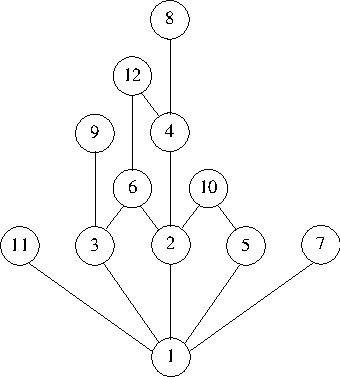
\includegraphics{figures/divi2.pdf}
\graphic{divi2}
\caption{A DAG whose Walk Relation is Divisibility on $\set{1,2,\dots,12}$.}
\label{fig:divisibility-DAG}
\end{figure}

If we're using a DAG to represent a partial order---so all we care
about is the the walk relation of the DAG---we could replace the DAG
with any other DAG with the same walk relation.  \fi
This raises the question of finding a DAG with the \emph{smallest}
number of edges that determines a given strict partial order.  For
\emph{finite} strict partial orders, the smallest such DAG turns out
to be unique and easy to find (see Problem~\ref{CP_covering_edges}).

\begin{problems}
\practiceproblems
\pinput{TP_The_Divisibility_DAG}
\pinput{TP_strictPOs_are_DAGs}

\classproblems
\pinput{CP_covering_edges}
\pinput{CP_tournament_chain}
\pinput{CP_tournament_graphs}
\pinput{CP_de_Bruijn_graphs}

\homeworkproblems
\pinput{PS_shortest_directed_closed_walk}
\pinput{CP_walk_relation_composition}  %renamed from PS_ but maybe better as PS_ after all
\pinput{PS_transitive_closure_proof}
%\pinput{PS_finite_transitive_closure}
\pinput{PS_odd_length_walk}
\pinput{PS_directed_Euler_circuits}
\pinput{PS_king_chicken}

\examproblems
\pinput{FP_partial_order_short_answer}

\end{problems}

\begin{editingnotes}
* add problem building on matrix rep to compute transitive closure
* add min, + shortest path matrix  multiplication
* likewise OR/AND matrix multiplication
\end{editingnotes}



\iffalse
\subsection{Weak Partial Orders}\label{partial_order_sec}

, but so is the containment relation on sets
and the divisibility relation on integers.
\fi

\iffalse

\section{Axioms for Partial Orders}

The prerequisite structure among MIT subjects provides a nice illustration
of partial orders.  Here is a table indicating some of the prerequisites of
subjects in the the Course 6 program of Spring '07:
\begin{center}
\begin{tabular}{|l|l|}
\hline
Direct Prerequisites & Subject\\ \hline
18.01 & 6.042\\ \hline
 18.01 & 18.02\\ \hline
 18.01 & 18.03\\ \hline
 8.01 & 8.02\\ \hline
 6.001 & 6.034\\ \hline
 6.042 & 6.046\\ \hline
 18.03, 8.02 & 6.002\\ \hline
 6.001, 6.002 & 6.004\\ \hline
 6.001, 6.002 & 6.003\\ \hline
 6.004 & 6.033\\ \hline
 6.033 & 6.857\\ \hline
 6.046 & 6.840\\ \hline
\end{tabular}
\end{center}

Since 18.01 is a direct prerequisite for 6.042, a student must take 18.01
before 6.042.  Also, 6.042 is a direct prerequisite for 6.046, so in fact,
a student has to take \emph{both} 18.01 and 6.042 before taking 6.046.  So
18.01 is also really a prerequisite for 6.046, though an implicit or
indirect one; we'll indicate this by writing
\[
18.01 \prq 6.046.
\]

This prerequisite relation has a basic property known as
\term{transitivity}: if subject $a$ is an indirect prerequisite of
subject $b$, and $b$ is an indirect prerequisite of subject $c$, then
$a$ is also an indirect prerequisite of $c$.

In this table, a longest sequence of prerequisites is
\[
18.01 \prq 18.03 \prq 6.002 \prq 6.004 \prq 6.033 \prq 6.857
\]
so a student would need at least six terms to work through this sequence
of subjects.  But it would take a lot longer to complete a Course 6 major
if the direct prerequisites led to a situation\footnote{MIT's Committee on
Curricula has the responsibility of watching out for such bugs that might
creep into departmental requirements.} where two subjects turned out to be
prerequisites of \emph{each other}!  So another crucial property of the
prerequisite relation is that if $a \prq b$, then it is not the case that
$b \prq a$.  This property is called \term{asymmetry}.

Another basic example of a partial order is the subset relation,
$\subseteq$, on sets.  In fact, we'll see that every partial order can be
represented by the subset relation.

\begin{definition}
A binary relation, $R$, on a set $A$ is:
\begin{itemize}

\item \emph{transitive} \qiff 
$[a \mrel{R}  b \text{ and } b \mrel{R}  c]\ \QIMPLIES\  a \mrel{R}  c$
\quad for every $a,b,c\in A$,

\item \emph{asymmetric} \qiff
$a \mrel{R}  b\  \QIMPLIES\  \QNOT(b \mrel{R}  a)$
\quad for all $a,b\in A$,

\item a \emph{strict partial order} iff it is transitive and asymmetric.
\end{itemize}

\end{definition}

So the prerequisite relation, $\prq$, on subjects in the MIT catalogue is
a strict partial order.  More familiar examples of strict partial orders
are the relation, $<$, on real numbers, and the proper subset relation,
$\subset$, on sets.
\fi

\subsection{Weak Partial Orders}
The less-than-or-equal relation, $\leq$, is at least as familiar as
the less-than strict partial order, and the ordinary containment
relation, $\subseteq$, is even more common than the proper containment
relation.  These are examples of \emph{weak partial orders}, which are
just strict partial orders with the additional condition that every
element is related to itself.  To state this precisely, we have to
relax the asymmetry property so it does not apply when a vertex is
compared to itself; this relaxed property is called
\term{antisymmetry}:

\begin{definition}\label{antis}
A binary relation, $R$, on a set $A$, is \term{antisymmetric} iff, for
all $a \neq b \in A$,
\[
a \mrel{R}  b\ \QIMPLIES\ \QNOT(b \mrel{R}  a)
\]

\end{definition}

Now we can give an axiomatic definition of weak partial orders that
parallels the definition of strict partial orders.\footnote{Some
  authors define partial orders to be what we call weak partial
  orders, but we'll use the phrase ``partial order'' to mean either a
  weak or strict one.}

\begin{definition}\label{def:weakPO-axiom}
A binary relation on a set is a \emph{weak partial order} iff it is
transitive, reflexive, and antisymmetric.
\end{definition}

The following lemma gives another characterization of weak partial
orders that follows directly from this definition.
\begin{lemma}
A relation $R$ on a set, $A$, is a weak partial order iff
there is a strict partial order, $S$, on $A$ such that
\[
a \mrel{R} b \qiff (a \mrel{S} b\ \QOR\ a = b),
\]
for all $a,b \in A$.
\end{lemma}

Since a length zero walk goes from a vertex to itself, this lemma
combined with Theorem~\ref{thm:SPOiffDAG} yields:
\begin{corollary}\label{weakPOiffDAGwalk}
A relation is a weak partial order iff it is the walk relation of a DAG.
\end{corollary}

For weak partial orders in general, we often write an ordering-style
symbol like $\preceq$ or $\sqsubseteq$ instead of a letter symbol like
$R$.\footnote{General relations are usually denoted by a letter like
  $R$ instead of a cryptic squiggly symbol, so $\preceq$ is kind of
  like the musical performer/composer Prince, who redefined the
  spelling of his name to be his own squiggly symbol.  A few years ago
  he gave up and went back to the spelling ``Prince.''}  Likewise, we
generally use $\prec$ or $\sqsubset$ to indicate a strict partial
order.

\begin{editingnotes}

We also write $b \succeq a$ to
mean $a \preceq b$ and $b \succ a$ to mean $a \prec b$.

\end{editingnotes}

Two more examples of partial orders are worth mentioning:

\begin{example}\label{supset}
Let $A$ be some family of sets and define $a \mrel{R} b$ iff $a
\supset b$.  Then $R$ is a strict partial order.
\end{example}

\iffalse
For integers, $m,n$ we write $m \divides n$ to mean that $m$
\emph{divides} $n$, namely, there is an integer, $k$, such that $n=km$.
\fi

\begin{example}\label{divides}
The divisibility relation is a weak partial order on the nonnegative integers.
\end{example}

\section{Representing Partial Orders by Set Containment}\label{poset-as-sets_sec}

Axioms can be a great way to abstract and reason about important
properties of objects, but it helps to have a clear picture of the
things that satisfy the axioms.  DAGs provide one way to picture
partial orders, but it also can help to picture them in terms of other
familiar mathematical objects.  In this section, we'll show that every
partial order can be pictured as a collection of sets related by
containment.  That is, every partial order has the ``same shape'' as
such a collection.  The technical word for ``same shape'' is
``isomorphic.''

\begin{definition}\label{relation-isomorphism}
  A binary relation, $R$, on a set, $A$, is
  \term{isomorphic} to a relation, $S$, on a set $B$ iff there is a
  relation-preserving bijection from $A$ to $B$; that is, there is
  a bijection $f:A \to B$ such that for all $a,a' \in A$,
  \[
  a \mrel{R} a'\ \qiff\ f(a) \mrel{S} f(a').
  \]
\end{definition}

To picture a partial order, $\preceq$, on a set, $A$, as a collection of
sets, we simply represent each element $A$ by the set of elements
that are $\preceq$ to that element, that is,
\[
a \corresp \set{b \in A \suchthat b \preceq a}.
\]
For example, if $\preceq$ is the divisibility relation on the set of
integers, $\set{1,3,4,6,8,12}$, then we represent each of these integers
by the set of integers in $A$ that divides it.  So
\begin{align*}
1 & \corresp \set{1}\\
3 & \corresp \set{1,3}\\
4 & \corresp \set{1,4}\\
6 & \corresp \set{1,3,6}\\
8 & \corresp \set{1,4,8}\\
12 & \corresp \set{1,3,4,6, 12}
\end{align*}
So, the fact that $3 \divides 12$ corresponds to the fact that $\set{1,3}
\subseteq \set{1,3,4,6, 12}$.

In this way we have completely captured the weak partial order $\preceq$ by the
subset relation on the corresponding sets.  Formally, we have
\begin{lemma}\label{rgb}
  Let $\preceq$ be a weak partial order on a set, $A$.  Then $\preceq$
  is isomorphic to the subset relation, $\subseteq$, on the collection
  of inverse images under the $\preceq$ relation of elements $a \in
  A$.
\end{lemma}
We leave the proof to
Problem~\ref{CP_weak_partial_order_isomorphic_to_subset}.  Essentially
the same construction shows that strict partial orders can be
represented by sets under the proper subset relation, $\subset$
(Problem~\ref{PS_strict_partial_order_isomorphic_to_subset}).  To
summarize:
\begin{theorem}
  Every weak partial order, $\preceq$, is isomorphic to the subset
  relation, $\subseteq$, on a collection of sets.

  Every strict partial order, $\prec$, is isomorphic to the proper
  subset relation, $\subset$, on a collection of sets.
\end{theorem}


\begin{problems}
\classproblems
\pinput{CP_prerequisite_relation}
\pinput{CP_partial_order_on_power_set}
\pinput{CP_weak_partial_order_isomorphic_to_subset}

\homeworkproblems
\pinput{PS_strict_partial_order_isomorphic_to_subset}

\begin{editingnotes}
Add a Sperner's Lemma problem?
\end{editingnotes}

\end{problems}


%% Total Orders %%%%%%%%%%%%%%%%%%%%%%%%%%%%%%%%%%%%%%%%%%%%%%%%%%%%%%%%%%%%%%%
\begin{editingnotes}
\TBA{REVISE} to use ``linear order'' language.  Explain that all the
elements in a linear order are ``lined up'' so that given any two, one
is in front of the other.  In a nonlinear partial order, elements
might be next to each other.
\end{editingnotes}

\section{Linear Orders}

The familiar order relations on numbers have an important additional
property: given two different numbers, one will be bigger than the
other.  Partial orders with this property are said to be \emph{linear
  orders}.  You can think of a linear order as one where all the
elements are lined up so that everyone knows exactly who is ahead and
who is behind them in the line.
\footnote{Linear orders are often called ``total'' orders, but this
  terminology conflicts with the definition of ``total relation,'' and
  it regularly confuses students.

  Being a linear order is a much stronger condition than being a
  partial order that is a total relation.  For example, any weak
  partial order is a total relation but generally won't be linear.}

\begin{definition}\label{def:path_total}
Let $R$ be a binary relation on a set, $A$, and let $a, b$ be elements of
$A$.  Then $a$ and $b$ are \emph{comparable} with respect to $R$ iff $[a
  \mrel{R} b\ \QOR\ b \mrel{R} a]$.  A partial order for which every two
different elements are comparable is called a \emph{linear order}.
\end{definition}

So $<$ and $\le$ are linear orders on $\reals$.  On the other hand, the
subset relation is \emph{not} linear, since, for example, any two different
finite sets of the same size will be incomparable under $\subseteq$.  The
prerequisite relation on Course 6 required subjects is also not linear
because, for example, neither 8.01 nor 6.042 is a prerequisite of the
other.

\iffalse
The name linear is based on the following
\begin{lemma}\label{path_total_lem} For any
  finite, nonempty set of vertices from a linear order, there is
  a directed path going through exactly these vertices.  If
  the digraph is a DAG, the directed path is unique.
\end{lemma}
Lemma~\ref{path_total_lem} is easy to prove by induction on the size
of the set of vertices.  The proof is given in
Problem~\ref{CP_tournament_chain}.
\fi

\begin{problems}
\practiceproblems
\pinput{TP_basic_partial_orders}
\pinput{TP_divisibility_partial_order}
\pinput{TP_transitive_irreflexive_implies_asymmetric}

\classproblems
\pinput{CP_partially_ordered_by_divisibility}
\pinput{CP_binary_relations_on_01}
\pinput{CP_inverse_partial_order}

\homeworkproblems
\pinput{PS_preserve_transitivity}

\examproblems
\pinput{CP_binary_relations_on_01_mq}

\end{problems}


%% Product Orders %%%%%%%%%%%%%%%%%%%%%%%%%%%%%%%%%%%%%%%%%%%%%%%%%%%%%%%%%%%%%
\section{Product Orders}\label{prodsec}

Taking the product of two relations is a useful way to construct new
relations from old ones.

\begin{definition}\label{productrel}
\hyperdef{def}{productrel}{The product}, $R_1 \cross R_2$, of relations
$R_1$ and $R_2$ is defined to be the relation with
\begin{eqnarray*}
\domain{R_1 \cross R_2} &\eqdef& \domain{R_1} \cross \domain{R_2},\\
\codomain{R_1 \cross R_2} &\eqdef& \codomain{R_1} \cross \codomain{R_2},\\
(a_1,a_2)\, (R_1 \cross R_2)\, (b_1,b_2) &\text{iff}& [a_1\, R_1\, b_1
\text{ and } a_2\, R_2\, b_2].
\end{eqnarray*}

\end{definition}

\begin{example}\label{Y}
Define a relation, $Y$, on age-height pairs of being younger \emph{and}
shorter.  This is the relation on the set of pairs $(y,h)$ where $y$ is a
nonnegative integer $\le 2400$ that we interpret as an age in months, and $h$
is a nonnegative integer $\le 120$ describing height in inches.  We define $Y$
by the rule
\[
(y_1,h_1)\, Y\, (y_2,h_2) \qiff y_1 \le y_2\ \QAND\ h_1 \le h_2.
\]
That is, $Y$ is the product of the $\le$-relation on ages and the
$\le$-relation on heights.
\end{example}

It follows directly from the definitions that products preserve the
properties of transitivity, reflexivity, irreflexivity, and
antisymmetry, as shown in
Problem~\ref{CP_product_relation_properties}.  If $R_1$ and
$R_2$ both have one of these properties, then so does $R_1 \cross
R_2$.  This implies that if $R_1$ and $R_2$ are both partial orders,
then so is $R_1 \cross R_2$.

On the other hand, the property of being a linear order is not preserved.
For example, the age-height relation $Y$ is the product of two linear
orders, but it is not linear: the age 240 months, height 68 inches pair,
(240,68), and the pair (228,72) are incomparable under $Y$.

\begin{problems}

\classproblems
\pinput{CP_product_relation_properties}

\end{problems}

\begin{editingnotes}
\chapter*{Well-founded partial orders}
omitted
\end{editingnotes}

\section{Equivalence Relations}\label{equiv_rel_sec}
\begin{definition}
A relation is an \term{equivalence relation} if it is reflexive,
symmetric, and transitive.
\end{definition}

Congruence modulo~$n$ is an important example of an equivalence
relation:
\begin{itemize}

\item
It is reflexive because $x \equiv x \pmod{n}$.

\item
It is symmetric because $x \equiv y \pmod{n}$ implies $y \equiv x
\pmod{n}$.

\item
It is transitive because $x \equiv y \pmod{n}$ and $y \equiv z
\pmod{n}$ imply that $x \equiv z \pmod{n}$.

\end{itemize}
There is an even more well-known example of an equivalence relation:
equality itself.

Any total function defines an equivalence relation on its domain:
\begin{definition}\label{equiv_f}
If $f:A \to B$ is a total function, define a relation $\equiv_f$ by the rule:
\[
a \equiv_f a'  \QIFF f(a) = f(a').
\]
\end{definition}
From its definition, $\equiv_f$ is reflexive, symmetric and transitive
because these are properties of equality.  That is, $\equiv_f$ is an
equivalence relation.  This observation gives another way to see that
congruence modulo~$n$ is an equivalence relation: the Remainder
Lemma~\ref{lem:conrem} implies that congruence modulo~$n$ is the same
as $\equiv_r$ where $r(a)$ is the remainder of $a$ divided by $n$.

In fact, a relation is an equivalence relation iff it equal $\equiv_f$
for some total function $f$ (see
Problem~\ref{CP_equivalence_same_property}).  So equivalence relations
could be been defined using Definition~\ref{equiv_f}.

\subsection{Equivalence Classes}

Equivalence relations are closely related to \idx{partitions} because
the images of elements under an equivalence relation are the blocks of
a partition.

\begin{definition}\label{def:equiv_class}
Given an equivalence relation $R : A \to A$, the \term{equivalence
  class},~$[a]_R$, of an element $a \in A$  is the set of all elements of~$A$
related to~$a$ by~$R$.  Namely,
\begin{equation*}
    [a]_R \eqdef \set{x \in A \suchthat a \mrel{R} x}.
\end{equation*}
\end{definition}
In other words, $[a]_R$ is the image $R(a)$.

For example, suppose that $A = \integers$ and $a \mrel{R} b$ means
that $a \equiv b \pmod{5}$.  Then
\begin{equation*}
    [7]_R = \set{\dots, -3, 2, 7, 12, 22, \dots}.
\end{equation*}
Notice that 7, 12, 17, etc., all have the same equivalence class; that
is, $[7]_R = [12]_R = [17]_R = \cdots$.

There is an exact correspondence between equivalence relations on~$A$
and partitions of~$A$.  Namely, given on one hand any partition of a
set, then being in the same block is obviously an equivalence
relation.  On the other hand we have:
\begin{theorem}\label{equiv-partition_thm}
The equivalence classes of an equivalence relation on a set~$A$ are
the blocks of a partition of~$A$.
\end{theorem}

We'll leave the proof of Theorem~\ref{equiv-partition_thm} as an easy
exercise in axiomatic reasoning (see
Problem~\ref{CP_equiv_partition_proof}), but let's look at an example.
The congruent-mod-5 relation partitions the integers into five
equivalence classes:
\begin{gather*}
    \set{ \dots, -5, 0, 5, 10, 15, 20, \dots } \\
    \set{ \dots, -4, 1, 6, 11, 16, 21, \dots } \\
    \set{ \dots, -3, 2, 7, 12, 17, 22, \dots } \\
    \set{ \dots, -2, 3, 8, 13, 18, 23, \dots } \\
    \set{ \dots, -1, 4, 9, 14, 19, 24, \dots }
\end{gather*}
In these terms, $x \equiv y \pmod{5}$ is equivalent to the assertion
that $x$ and~$y$ are both in the same block of this partition.  For
example, $6 \equiv 16 \pmod{5}$, because they're both in the second
block, but $2 \not\equiv 9 \pmod{5}$ because 2~is in the third block
while 9~is in the last block.

In social terms, if ``likes'' were an equivalence relation, then
everyone would be partitioned into cliques of friends who all like
each other and no one else.

\begin{problems}
\practiceproblems
\pinput{TP_Equivalence_relations}
\pinput{TP_basic_relations}

\classproblems
\pinput{CP_equiv_partition_proof}
\pinput{CP_equivalence_same_property}

\homeworkproblems
\pinput{PS_equivalence_relation_operations}

\end{problems}

\section{Summary of Relational Properties}\label{prop_summary_sec}

A relation $R: A \to A$ is the same as a digraph with vertices $A$.

\begin{description}

\item[Reflexivity]

$R$ is \term{reflexive} when
\[
\forall x \in A. \; x \mrel{R} x.
\]

%``Everyone likes themselves.''

Every vertex in~$R$ has a self-loop.

\item[Irreflexivity]

$R$ is \term{irreflexive} when
\[
\QNOT[ \exists x \in A. \; x \mrel{R} x].
\]

%``No one likes themselves.''

There are no self-loops in~$R$.

\item[Symmetry]

$R$ is \term{symmetric} when
\[
\forall x, y \in A. \; x \mrel{R} y \QIMP y \mrel{R} x.
\]

%``If $x$ likes~$y$, then $y$ likes~$x$.''

If there is an edge from $x$ to~$y$ in~$R$, then there is an edge back
from $y$ to~$x$ as well.

\item[Asymmetry]
$R$ is \emph{asymmetric} when
\[
\forall x, y \in A. \; x \mrel{R} y \QIMPLIES \QNOT( y \mrel{R} x ).
\]
There is at most one directed edge between any two vertices in $R$,
and there are no self-loops.

\item[Antisymmetry]
$R$ is \term{antisymmetric} when
\[
\forall x \neq y \in A. \; x \mrel{R} y \QIMPLIES \QNOT( y \mrel{R} x ).
\]
Equivalently,
\[
\forall x, y \in A. \; (x \mrel{R} y \QAND\ y \mrel{R} x ) \QIMPLIES\ x = y.
\]

There is at most one directed edge between any two distinct vertices,
but there may be self-loops.

\item[Transitivity]
$R$ is \term{transitive} when
\[
 \forall x, y, z \in A. \; (x \mrel{R} y \QAND y \mrel{R} z) \QIMPLIES x \mrel{R} z.
\]
%``If $x$ likes~$y$ and $y$ likes~$z$, then $x$ likes~$z$ too.''

If there is a positive length path from~$u$ to~$v$, then there is an edge from~$u$ to~$v$.

\iffalse
For any walk $v_0, v_1, \dots, v_k$ in~$G$ where $k \ge 2$,
$\diredge{v_0}{v_k}$ is in~$G$ (and, hence, $\diredge{v_i}{v_j}$ is
also in~$G$ for all $i < j$.
\fi

\item[Linear] $R$ is \term{linear} when
\[
 \forall x \neq y \in A. \; (x \mrel{R} y\ \QOR\ y \mrel{R} x)
\]
Given any two vertices in $R$, there is an edge in one direction or the
other between them.

For any finite, nonempty set of vertices of $R$, there is a directed path
going through exactly these vertices.

\item[Strict Partial Order] $R$ is a \term{strict partial order} iff
  $R$ is transitive and irreflexive iff $R$ is transitive and
  asymmetric iff it is the positive length walk relation of a DAG.
  
\item[Weak Partial Order] $R$ is a \term{weak partial order} iff $R$ is
  transitive and anti-symmetric and reflexive iff $R$ is the walk
  relation of a DAG.

\item[Equivalence Relation] $R$ is an \term{equivalence relation} iff $R$
  is reflexive, symmetric and transitive iff $R$ equals the
  \emph{in-the-same-block}-relation for some partition of $\domain{R}$.

\end{description}

\endinput

